\section{Deep Reinforcement Learning}

\subsection{Reinforcement Learning}

强化学习要解决的问题类似于玩一个游戏：Environment 告诉 Agent 当前状态 $s_t$，Agent 据此做出一个动作 $a_t$，Environment 为该动作给出 $r_t$ 的奖励，并更新状态为 $s_{t+1}$，然后反复上述过程。

\begin{figure}[H]
    \centering
    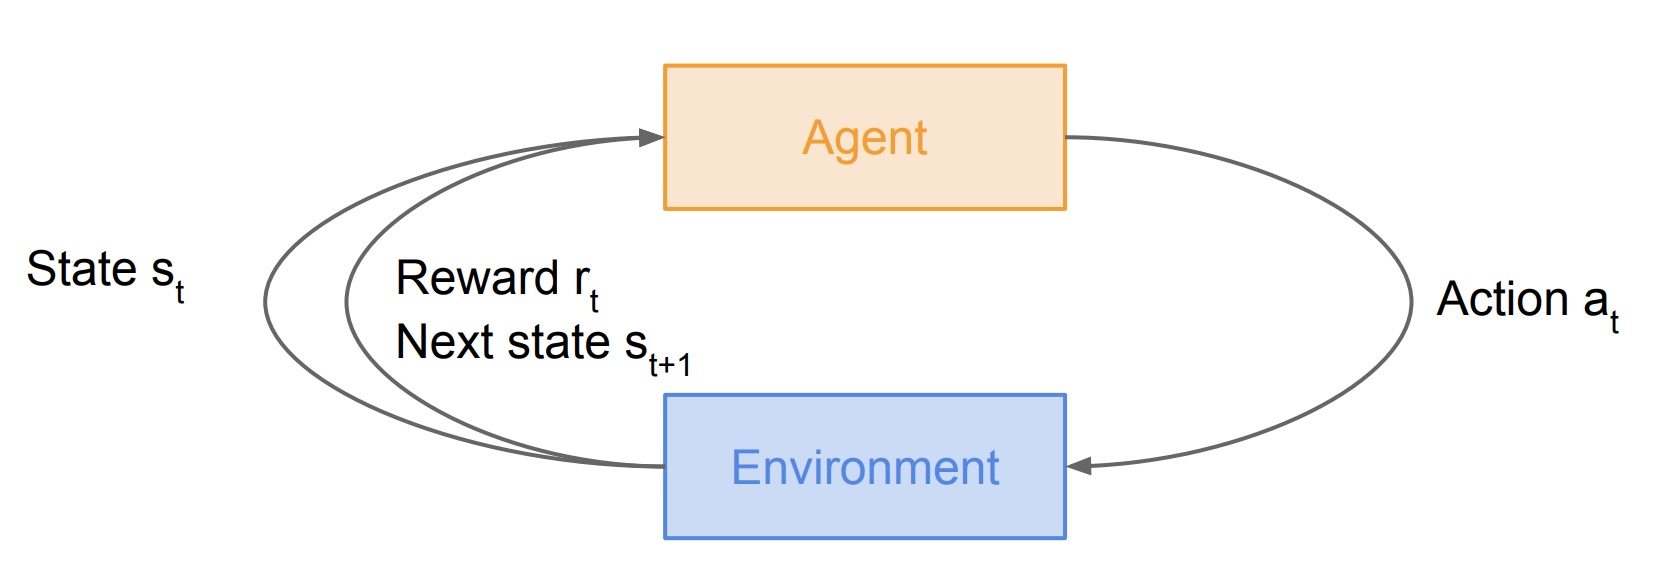
\includegraphics[width=0.6\linewidth]{figs/chapter9/rl.jpg}
\end{figure}

\subsection{Markov Decision Process}

强化学习可以用马尔可夫过程进行数学形式化的表述，因为它满足 \textbf{Markov property}，即当前状态完全定义了未来的状态，或者说未来的状态仅受当前状态、而不受过去状态的影响。

马尔可夫过程定义为：$(\mathcal S,\mathcal A,\mathcal R,\mathbb P,\gamma)$，其中 $\mathcal S$ 表示所有可能的状态集合，$\mathcal A$ 表示所有可能的动作集合，$\mathcal R$ 表示奖励在给定 $\mathcal S$ 和 $\mathcal A$ 下的分布，$\mathbb P$ 表示状态的转移概率，$\gamma$ 是 discount factor，用于对近期奖励和远期奖励进行加权。

马尔可夫过程的流程是：

\begin{itemize}
    \item 在 $t=0$ 时刻，environment 对初始状态进行采样 $s_0\sim p(s_0)$；
    \item 接下来，反复执行以下步骤直到结束：
    \begin{itemize}
        \item Agent 选择动作 $a_t$；
        \item Environment 对奖励进行采样 $r_t\sim \mathcal R(\bullet\mid s_t,a_t)$；
        \item Environment 对下一个状态进行采样 $s_{t+1}\sim\mathbb P(\bullet\mid s_t,a_t)$；
        \item Agent 收到奖励 $r_t$ 和下一个状态 $s_{t+1}$。

    \end{itemize}
\end{itemize}
一个决策 $\pi$ 就是一个从 $\mathcal S$ 到 $\mathcal A$ 的函数，决定在每一个状态下执行什么动作，而我们的目标就是找到最佳的决策 $\pi^*$ 以使得累计奖励 $\sum_{t\geqslant 0}\gamma^t r_t$ 最大。但是，由于我们的众多变量都是随机变量，所以我们实际上要最大化的是累计奖励的期望，即：
\[
\pi^*=\arg\max_\pi\mathbb E\left[\sum_{t\geqslant0}\gamma^tr_t\mid \pi\right]
\]
其中 $s_0\sim p(s_0),\,a_t\sim\pi(\bullet\mid s_t),\,s_{t+1}\sim \mathbb P(\bullet\mid s_t,a_t)$.

服从一个决策将会产生一个样本路径（轨迹）：$s_0,a_0,r_0,s_1,a_1,r_1,\ldots$，我们需要一种方式量化从这个初始状态 $s_0$ 开始的好坏程度，因此定义 \textbf{value function}：
\[
V^{\pi}(s)=\mathbb E\left[\sum_{t\geqslant 0}\gamma ^tr_t\mid s=s_0,\pi\right]
\]
进一步的，我们还可以定义从初始状态 $s_0$ 和初始动作 $a_0$ 开始服从某一个决策 $\pi$ 的好坏程度，称为 \textbf{Q-value function}：
\[
Q^{\pi}(s,a)=\mathbb E\left[\sum_{t\geqslant 0}\gamma^tr_t\mid s_0=s,a_0=a,\pi\right]
\]
那么，最佳的 Q-value function $Q^*$ 就是在给定 $(s,a)$ 下找到使得 $Q^{\pi}(s,a)$ 最大的决策方式 $\pi$：
\[
Q^*(s,a)=\max_\pi\mathbb E\left[\sum_{t\geqslant 0}\gamma^tr_t\mid s_0=s,a_0=a,\pi\right]
\]
而一个核心的等式——\textbf{Bellman Equation} 告诉我们 $Q^*$ 满足：
\[
Q^*(s,a)=\mathbb E_{s'\sim \mathcal E}\left[r+\gamma\max_{a'}Q^*(s',a')\mid s,a\right]
\]

\begin{com}
    推导：
    \begin{align*}
    Q^\pi(s,a)&=\mathbb E\left[r_{t}+\gamma r_{t+1}+\gamma^2r_{t+2}+\cdots\mid s_0=s,a_0=a,\pi\right]\\
    &=\mathbb E[r_t+\gamma(r_{t+1}+\gamma r_{t+2}+\cdots)\mid s_0=s,a_0=a,\pi]\\
    &=\mathbb E[r_t+\gamma Q^{\pi}(s',a')\mid s_0=s,a_0=a,\pi]
    \end{align*}
    其中，$s',a'$ 是下一时刻的状态和动作。因此，$Q^\pi(s,a)$ 最大值就是当前奖励 $r_t$ 加上在接下来的状态中用最佳的动作得到的最大收益。
\end{com}

为了求解上述最佳 Q-value functino $Q^*$，根据 Bellman Equation，我们可以迭代求解，迭代格式为：
\[
Q_{i+1}(s, a)=\mathbb E\left[r+\gamma \max_{a'}Q_i(s',a')\mid s,a\right]
\]
可以证明，该迭代格式收敛到 $Q^*$.

这么做理论上可行，但是实际中我们需要遍历所有可能的 $(s,a)$ 对，这是不可行的。为了解决这个问题，我们可以找一个函数去近似 $Q(s,a)$，比如用一个神经网络——这就引出了 Q-Learning。

\subsection{Q-Learning}

正如前文所述，Q-Learning 的目的是用一个神经网络近似 $Q^*(s,a)$，即：
\[
Q(s,a;\theta)\approx Q^*(s,a)
\]
其中 $\theta$ 是我们的网络的参数。

要训练这个网络，关键是定义损失函数。由于 $Q^*$ 需要满足 Bellman Equation，我们可以用当前网络到 Bellman Equation 的 MSE 误差作为损失函数：
\begin{align*}
&L_i(\theta_i)=\mathbb E_{s,a\sim \rho(\bullet)}\left[(y_i-Q(s,a;\theta_i))^2\right]\\
\text{where}\;\;&y_i=\mathbb E_{s\sim \mathcal{E}}\left[r+\gamma\max_{a'}Q(s',a';\theta_{i-1})\mid s,a\right]
\end{align*}
在训练玩游戏时，一个自然的想法是用最近的若干连续的画面帧作为神经网络的输入，但这么做将会导致一些问题：首先这些样本将高度相关，以至于学习的效率低；其次，当前网络的参数将决定接下来输入样本的分布，例如当前的动作是向左走，那么接下来的训练样本将大量采样自画面左侧。为了解决这些问题，我们使用 \textbf{experience replay}：维护一个 replay memory table，其存储的是 $(s_t,a_t,r_t,s_{t+1})$ 组，在训练过程中不断更新其内容；在训练时，一个 minibatch 是从这个 table 中随机选取的，而非采取若干连续的状态，这样就解决了上述问题。

\subsection{Policy Gradients}

Q-Learning 的问题在于 Q-function 可以非常复杂，而我们需要的策略可能仅仅是一个非常简单的动作而已。这就引出了 Policy Gradients.

首先，我们定义决策空间为：$\Pi=\{\pi_\theta,\theta\in\mathbb R^m\}$. 对每个决策，我们定义其值为：
\[
J(\theta)=\mathbb E\left[\sum_{t\geqslant 0}\gamma^tr_t\mid \pi_\theta\right]
\]
我们的目标是最大化 $J(\theta)$，即找到 $\theta^*=\arg\max\limits_\theta J(\theta)$. 容易想到我们对 $\theta$ 做梯度上升即可。

$J(\theta)$ 可写作：
\[
J(\theta)=\mathbb E_{\tau\sim p(\tau;\theta)}[r(\tau)]=\int_\tau r(\tau)p(\tau;\theta)\mathrm d\tau
\]
其中 $\tau=(s_0,a_0,r_0,s_1,\ldots)$ 是一个决策轨迹，$r(\tau)$ 为其奖励。现在我们求解其梯度：
\begin{align*}
\nabla_\theta J(\theta)&=\int_\tau r(\tau)\nabla_\theta p(\tau;\theta)\mathrm d\tau\\
&=\int_\tau r(\tau) p(\tau;\theta)\nabla_\theta\ln p(\tau;\theta)\mathrm d\tau\\
&=\mathbb E_{\tau\sim p(\tau;\theta)}[r(\tau)\nabla_\theta\ln p(\tau;\theta)]
\end{align*}
由于 $p(\tau;\theta)=\prod\limits_{t\geqslant0}p(s_{t+1}\mid s_t,a_t)\pi_\theta(a_t\mid s_t)$，故：
\[
\nabla_\theta \ln p(\tau;\theta)=\nabla_\theta \sum_{t\geqslant 0}\ln p(s_{t+1}\mid s_t,a_t)+\ln \pi_\theta(a_t\mid s_t)=\nabla_\theta \sum_{t\geqslant 0}\ln\pi_\theta(a_t\mid s_t)
\]
于是乎，我们可以对轨迹 $\tau$ 进行采样，然后计算：
\[
\nabla_\theta J(\theta)\approx\sum_{t\geqslant 0}r(\tau)\nabla_\theta \ln\pi_\theta(a_t\mid s_t)
\]
但是这个 gradient estimator 很难达到我们想要的效果，因为其方差很大。为此，人们提出了若干减小方差的方法：

\begin{itemize}
    \item Idea 1：
    \[
    \nabla_\theta J(\theta)\approx \sum_{t\geqslant 0}\left(\sum_{t'\geqslant t} r_{t'}\right)\nabla_\theta\ln\pi_\theta(a_t\mid s_t)
    \]
    用从当前决策开始直到结束的过程中得到的奖励代替 $r(\tau)$。

    \item Idea 2：
    \[
    \nabla_\theta J(\theta)\approx \sum_{t\geqslant 0}\left(\sum_{t'\geqslant t} \gamma^{t'-t}r_{t'}\right)\nabla_\theta\ln\pi_\theta(a_t\mid s_t)
    \]
    加入一个 discount factor $\gamma$.

    \item Idea：引入 baseline function：
    \[
    \nabla_\theta J(\theta)\approx \sum_{t\geqslant 0}\left(\sum_{t'\geqslant t} \gamma^{t'-t}r_{t'}-b(s_t)\right)\nabla_\theta\ln\pi_\theta(a_t\mid s_t)
    \]

\end{itemize}
如何选取 baseline 呢？一个最简单的方法是取已经遍历过的决策轨迹的奖励的移动平均。不过利用 Q-value function，我们能得到更好的 baseline：
\[
\nabla_\theta J(\theta)\approx \sum_{t\geqslant 0}\left(Q^{\pi_\theta}(s_t,a_t)-V^{\pi_\theta}(s_t)\right)\nabla_\theta\ln\pi_\theta(a_t\mid s_t)
\]
直观上讲，我们希望 $A^{\pi_\theta}(s_t,a_t)=Q^{\pi_\theta}(s_t,a_t)-V^{\pi_\theta}(s_t)$ 越大越好，因为这表示我们选取的动作 $a_t$ 使得这之后我们得到的奖励期望值大于随便取一个动作得到的奖励期望值，我们称 $A^\pi(s,a)$ 为 \textbf{advantage function.}

现在我们得到了 Actor-Critic Algorithm，即结合 Policy Gradients 和 Q-learning 的算法：同时训练一个 actor，即决策，和 critic，即 Q-function——Actor 决定做一个动作，critic 告诉它这个动作的优劣以及应该如何调整；同时 critic 无需对所有 $(s,a)$ 对进行学习，而只需要学习 actor 做出的那些决策。
